%! TeX root = ../main.tex
\chapter{METODOLOGI}
\label{chap:metodologi}

% Ubah bagian ini sesuai dengan metodologi penelitian proposal / tugas akhir Anda.

\section{Diagram Alir Penelitian}
\label{sec:diagramalir}

Metodologi penelitian ini dilakukan melalui tahapan sebagaimana ditunjukkan pada Gambar~\ref{fig:alir-metodologi}. Penelitian dimulai dengan studi literatur dan identifikasi kebutuhan serta batasan sistem, kemudian dilanjutkan dengan perancangan sistem dan prototipe. Setelah itu, dilakukan implementasi pemrosesan, pengujian sistem, analisis data hasil pengujian, dan diakhiri dengan penarikan kesimpulan.

\begin{figure}[H]
  \centering
  % Ganti berkas gambar di bawah ini dengan diagram alir penelitian Anda di folder gambar/
  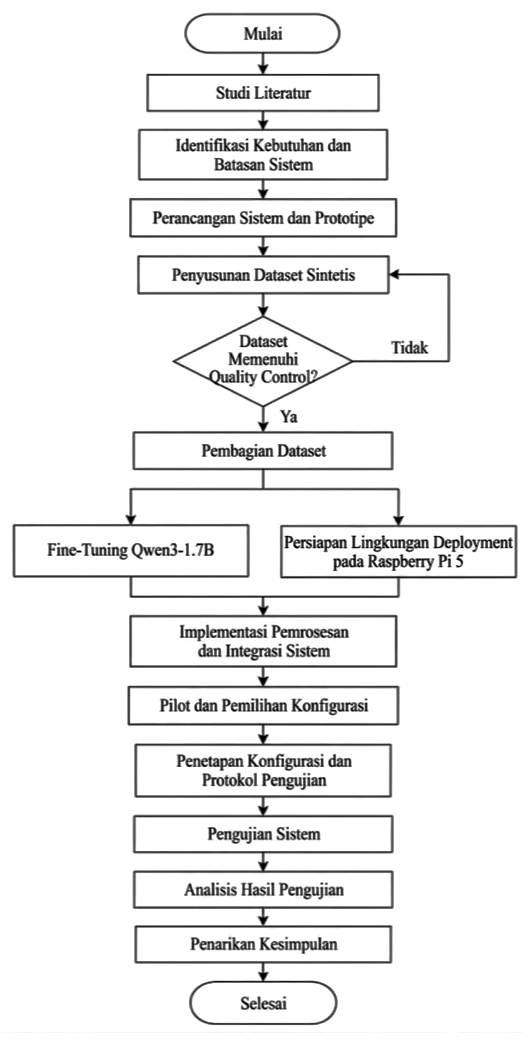
\includegraphics[height=13.5cm]{gambar/gambar-3-1.png}
  \caption{Diagram Alir Metodologi Penelitian}
  \label{fig:alir-metodologi}
\end{figure}

\section{Studi Literatur dan Identifikasi Kebutuhan}
\label{sec:studiliteratur}

\lipsum[1-2]

\section{Perancangan Sistem dan Prototipe}
\label{sec:perancangansistem}

\subsection{Arsitektur dan Diagram Blok Kerja}
\label{subsec:arsitektursistem}

Sistem dirancang dengan alur kerja yang menghubungkan setiap modul dari akuisisi data, prapemrosesan, pemrosesan utama, hingga tampilan antarmuka pengguna. Hubungan antarblok sistem dan aliran data ditunjukkan pada Gambar~\ref{fig:blok-sistem}.

\begin{figure}[H]
  \centering
  % Ganti berkas gambar di bawah ini dengan diagram blok kerja Anda di folder gambar/
  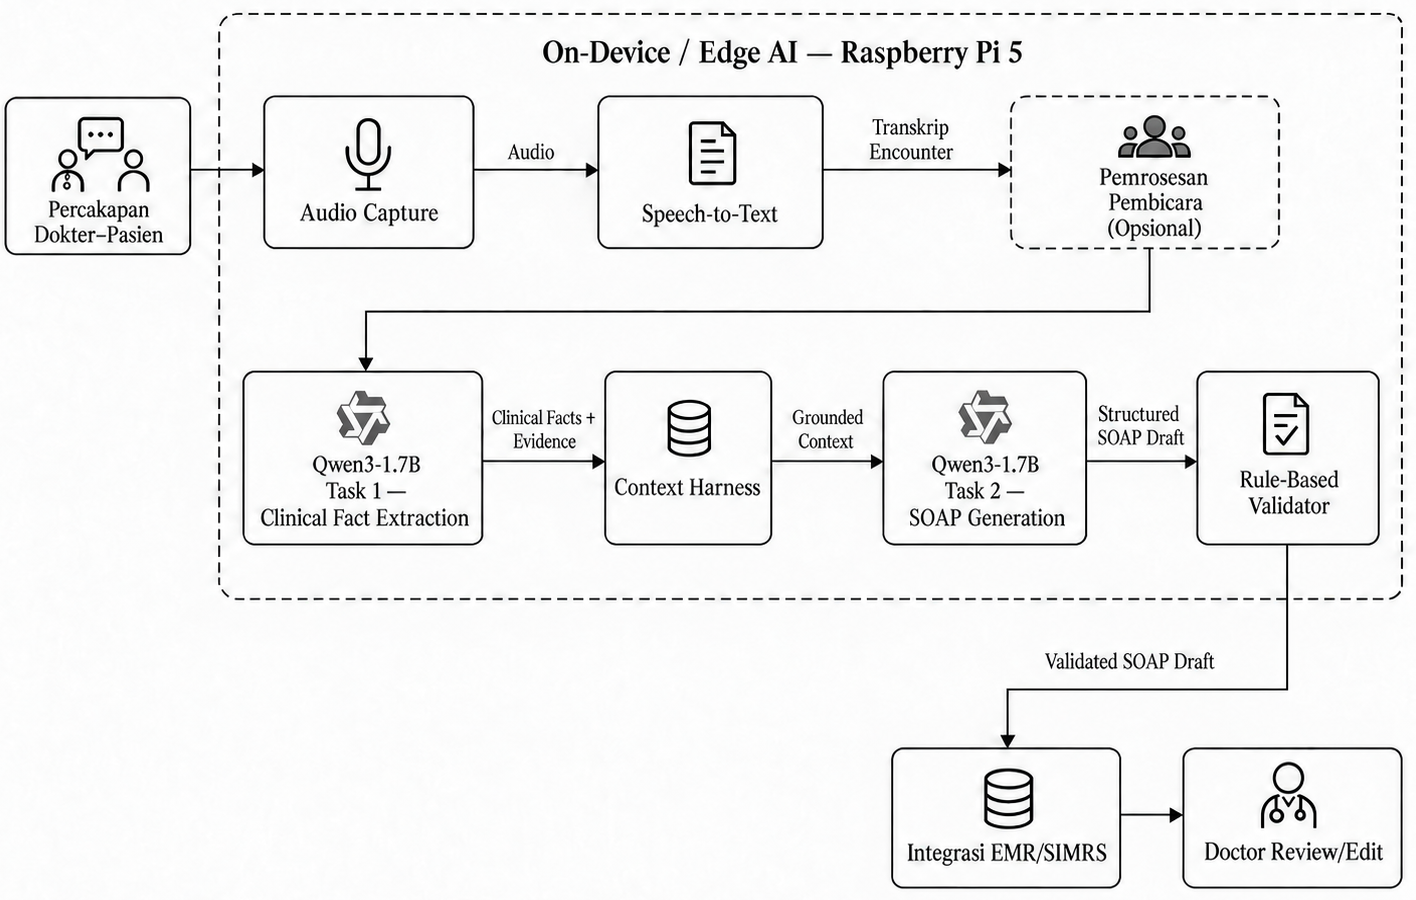
\includegraphics[width=\textwidth]{gambar/gambar-3-2.png}
  \caption{Diagram Blok Kerja Sistem}
  \label{fig:blok-sistem}
\end{figure}

\subsection{Perancangan Perangkat Keras dan Perangkat Lunak}
\label{subsec:perangkat}

\lipsum[3-4]

\section{Protokol Pengujian dan Evaluasi}
\label{sec:protokolpengujian}

\lipsum[5]

\section{Linimasa dan Jadwal Pelaksanaan}
\label{sec:linimasa}

\lipsum[6]
